\RequirePackage[l2tabu,orthodox]{nag}
\documentclass[11pt,letterpaper]{article}
\usepackage[T1]{fontenc}
\usepackage[utf8]{inputenc}
\usepackage{crimson}
\usepackage{helvet}
\usepackage[strict,autostyle]{csquotes}
\usepackage[USenglish]{babel}
\usepackage{microtype}
\usepackage{authblk}
\usepackage{booktabs}
\usepackage{caption}
\usepackage{endnotes}
\usepackage{geometry}
\usepackage{graphicx}
\usepackage{hyperref}
\usepackage{natbib}
\usepackage{rotating}
\usepackage{setspace}
\usepackage{titlesec}
\usepackage{url}
\usepackage{soul}
\usepackage[dvipsnames]{xcolor}
\usepackage[many]{tcolorbox}
\newtcolorbox{mybox}{colback = black!5!gray!50, colframe = black!75!black, segmentation style={solid}} % create text box
\usepackage{hanging}

% location of figure files, via graphicx package
\graphicspath{{./figures/}}

% configure the page layout, via geometry package
\geometry{
	paper=letterpaper,
	top=4cm,
	bottom=4cm,
	left=4cm,
	right=4cm}
\setstretch{1.02}
\clubpenalty=10000
\widowpenalty=10000

% set section/subsection headings as the sans serif font
\titleformat{\section}{\normalfont\sffamily\large\bfseries}{\thesection.}{0.3em}{}
\titleformat{\subsection}{\normalfont\sffamily\small\bfseries}{\thesubsection.}{0.3em}{}

% make figure/table captions sans-serif small font
\captionsetup{font={footnotesize,sf},labelfont=bf,labelsep=period}

% configure pdf metadata and link handling
\hypersetup{
	pdfauthor={Francisco Rowe, Robin Lovelace, Adam Dennett},
	pdftitle={Spatial Interaction Modelling: A Manisfesto},
	pdfsubject={Spatial Interaction Modelling: A Manisfesto},
	pdfkeywords={Spatial interaction modelling, Gravity modelling, Machine learning, Geographic data science},
	pdffitwindow=true,
	breaklinks=true,
	colorlinks=false,
	pdfborder={0 0 0}}

\title{Spatial Interaction Modelling: A Manisfesto\footnote{\textbf{Citation}: Rowe, F. Lovelace, R. Dennett, A., 2022. Spatial Interaction Modelling: A Manisfesto. In: Wolf, L., Heppenstall, A., and Harris, R. (eds) Edward Elgar Books}}
\author[1]{Francisco Rowe \thanks{\textit{Email}: F.Rowe-Gonzalez@liverpool.ac.uk}}
\affil[1]{Geographic Data Science Lab, Department of Geography and Planning, University of Liverpool, Liverpool, United Kingdom}
\author[2]{Robin Lovelace \thanks{\textit{Email}: R.Lovelace@leeds.ac.uk}}
\affil[2]{Institute for Transport Studies, University of Leeds, Leeds, United Kingdom}
\author[3]{Adam Dennett \thanks{\textit{Email}: a.dennet@ucl.ac.uk}}
\affil[3]{The Bartlett Centre for Advanced Spatial Analytics, University College London, London, United Kingdom}

\date{}

% From pandoc:
% https://github.com/jgm/pandoc-templates/blob/master/default.latex
\newlength{\cslhangindent}
\setlength{\cslhangindent}{1.5em}
\newlength{\csllabelwidth}
\setlength{\csllabelwidth}{3em}
\newlength{\cslentryspacingunit} % times entry-spacing
\setlength{\cslentryspacingunit}{\parskip}
\newenvironment{CSLReferences}[2] % #1 hanging-ident, #2 entry spacing
 {% don't indent paragraphs
  \setlength{\parindent}{0pt}
  % turn on hanging indent if param 1 is 1
  \ifodd #1
  \let\oldpar\par
  \def\par{\hangindent=\cslhangindent\oldpar}
  \fi
  % set entry spacing
  \setlength{\parskip}{#2\cslentryspacingunit}
 }%
 {}
\usepackage{calc}
\newcommand{\CSLBlock}[1]{#1\hfill\break}
\newcommand{\CSLLeftMargin}[1]{\parbox[t]{\csllabelwidth}{#1}}
\newcommand{\CSLRightInline}[1]{\parbox[t]{\linewidth - \csllabelwidth}{#1}\break}
\newcommand{\CSLIndent}[1]{\hspace{\cslhangindent}#1}
\setlength{\emergencystretch}{3em} % prevent overfull lines
\providecommand{\tightlist}{%
  \setlength{\itemsep}{0pt}\setlength{\parskip}{0pt}}

% https://stackoverflow.com/questions/41052687/rstudio-pdf-knit-fails-with-environment-shaded-undefined-error
\usepackage{color}
\usepackage{fancyvrb}
\newcommand{\VerbBar}{|}
\newcommand{\VERB}{\Verb[commandchars=\\\{\}]}
\DefineVerbatimEnvironment{Highlighting}{Verbatim}{commandchars=\\\{\}}
% Add ',fontsize=\small' for more characters per line
\usepackage{framed}
\definecolor{shadecolor}{RGB}{248,248,248}
\newenvironment{Shaded}{\begin{snugshade}}{\end{snugshade}}
\newcommand{\AlertTok}[1]{\textcolor[rgb]{0.94,0.16,0.16}{#1}}
\newcommand{\AnnotationTok}[1]{\textcolor[rgb]{0.56,0.35,0.01}{\textbf{\textit{#1}}}}
\newcommand{\AttributeTok}[1]{\textcolor[rgb]{0.77,0.63,0.00}{#1}}
\newcommand{\BaseNTok}[1]{\textcolor[rgb]{0.00,0.00,0.81}{#1}}
\newcommand{\BuiltInTok}[1]{#1}
\newcommand{\CharTok}[1]{\textcolor[rgb]{0.31,0.60,0.02}{#1}}
\newcommand{\CommentTok}[1]{\textcolor[rgb]{0.56,0.35,0.01}{\textit{#1}}}
\newcommand{\CommentVarTok}[1]{\textcolor[rgb]{0.56,0.35,0.01}{\textbf{\textit{#1}}}}
\newcommand{\ConstantTok}[1]{\textcolor[rgb]{0.00,0.00,0.00}{#1}}
\newcommand{\ControlFlowTok}[1]{\textcolor[rgb]{0.13,0.29,0.53}{\textbf{#1}}}
\newcommand{\DataTypeTok}[1]{\textcolor[rgb]{0.13,0.29,0.53}{#1}}
\newcommand{\DecValTok}[1]{\textcolor[rgb]{0.00,0.00,0.81}{#1}}
\newcommand{\DocumentationTok}[1]{\textcolor[rgb]{0.56,0.35,0.01}{\textbf{\textit{#1}}}}
\newcommand{\ErrorTok}[1]{\textcolor[rgb]{0.64,0.00,0.00}{\textbf{#1}}}
\newcommand{\ExtensionTok}[1]{#1}
\newcommand{\FloatTok}[1]{\textcolor[rgb]{0.00,0.00,0.81}{#1}}
\newcommand{\FunctionTok}[1]{\textcolor[rgb]{0.00,0.00,0.00}{#1}}
\newcommand{\ImportTok}[1]{#1}
\newcommand{\InformationTok}[1]{\textcolor[rgb]{0.56,0.35,0.01}{\textbf{\textit{#1}}}}
\newcommand{\KeywordTok}[1]{\textcolor[rgb]{0.13,0.29,0.53}{\textbf{#1}}}
\newcommand{\NormalTok}[1]{#1}
\newcommand{\OperatorTok}[1]{\textcolor[rgb]{0.81,0.36,0.00}{\textbf{#1}}}
\newcommand{\OtherTok}[1]{\textcolor[rgb]{0.56,0.35,0.01}{#1}}
\newcommand{\PreprocessorTok}[1]{\textcolor[rgb]{0.56,0.35,0.01}{\textit{#1}}}
\newcommand{\RegionMarkerTok}[1]{#1}
\newcommand{\SpecialCharTok}[1]{\textcolor[rgb]{0.00,0.00,0.00}{#1}}
\newcommand{\SpecialStringTok}[1]{\textcolor[rgb]{0.31,0.60,0.02}{#1}}
\newcommand{\StringTok}[1]{\textcolor[rgb]{0.31,0.60,0.02}{#1}}
\newcommand{\VariableTok}[1]{\textcolor[rgb]{0.00,0.00,0.00}{#1}}
\newcommand{\VerbatimStringTok}[1]{\textcolor[rgb]{0.31,0.60,0.02}{#1}}
\newcommand{\WarningTok}[1]{\textcolor[rgb]{0.56,0.35,0.01}{\textbf{\textit{#1}}}}


\begin{document}

\maketitle


\textbf{NOTE} This is a preprint version of the chapter. Please do not redistribute without
permission of the authors. You can get in touch with Francisco Rowe at
F.Rowe-Gonzalez@liverpool.ac.uk; Robin Lovelace at R.Lovelace@leeds.ac.uk or Adam Dennett a.dennet@ucl.ac.uk

\begin{abstract}


%\vspace{1cm}
\end{abstract}



\pagebreak

Overall aim: To set our view about how the field of spatial interaction modelling should evolve.

Key argument: Spatial interaction models are great, yet, not progress has been made over the last two/three decades (though we should recognise the work LeSage on spatial econometrics, Dan Griffith on spatial filtering, Kanaroglou et al on spatial discrete choice modelling, radiation models).
Key challenges have prevented progress:

1.
reproducibility

2.
calibration

3.
large volumes of granular spatial data .

Context: spatial interaction modelling in a world of big data, machine learning, open science, digital technology and uncertainty.

The text included here is for our own benefit.
The idea of challenges

\hypertarget{definition-and-uses}{%
\section{Definition and Uses}\label{definition-and-uses}}

For over 70 years, spatial interaction models (SIMs) have been the workmodel to understand spatial interactions between entities at different locations in physical space.
SIMs represent mathematical formulations through which the spatial interaction between geographic places through flows of people, information and goods can be represented.
Intuitively, these models seek to represent the spatial interaction between places as a function of three components: origin characteristics, destination characteristics and the separation between origins and destinations.
Originally adapted from physics, spatial flows between an origin and a destination were concieved to be proportional to their gravitational force and inversely related to their spatial separation.
Characteristics of origins and destinations are used to represent gravitational forces pushing and/or pulling people, information and goods from and to specific locations, and different forms of distance and cost are used to represent the deterring effects of spatial separation on spatial flows.

SIMs have been instrumental and applied in a wide range of contexts to support data analysis and decision making in retail, transport, housing, epidemiology, public health, land use, urban and population modelling and planningprojection and forecasting contexts.
SIMs are generally used for two key purposes.
A key purpose is the \emph{prediction} of the size and direction of spatial flows.
SIMs have been widely used to predict the impact of the development of new service units, such as shopping stores, healthcare facilities and housing units on the potential demand for associated services and traffic patterns.
Predictions from such analyses enable the identification of optimal locations and size for potential new service units.
A second key purpose of SIMs is \emph{inference} about the factors shaping the spatial interactions in a network of flows.
SIMs have been used to determine and understand the influence of retail store on consumers' store choices and place attributes on migration decisions and commuting patterns.
SIMs have also been used to delineate geographical areas of service and retail catchment areas.

Formally SIMs take different forms.
Newtonian gravity models are probably the most widely known and used in social sciences.
Adapted from physics, the basic gravity model assumes that the interactions \(T_{i j}\) between an origin \(i\) and a destination \(j\) in the form of flows can be understood as a function of driving forces like masses \(V_{i}\) and \(W_{j}\) , and a measure of spatial separation \(c_{ij}\) .
Areas are assumed to interact in a positively reinforcing way that is multiplicative of their masses, and at the same time their interactions are expected to diminish with the intervening role of spatial separation.
Spatial separation is generally measured by distance, cost or time involved in the interaction, and is often represented by a distance-decay function.
The model also requires a \(k\) factor to proportionality between expected and observed flows, and \(\beta\) parameter representing the deterring effect of spatial separation, or distance.
The key task in a gravity model is to estimate these parameters.
A typical notation for the model is:

\[
T_{i j}=k \frac{V_{i} W_{j}}{c_{i j}^{\beta}}
\]

In practice, a matrix of flows between a set of origins, a set of destinations and a measure of spatial separation between origins and destinations is the key input for SIMs.
A family of SIMs taking four distinctive shapes is typically considered (Wilson 1971).
A \emph{unconstrained} formulation of the model to ensure that the total sum of the predicted flows from a gravity model be equal the total sum of the observed flows across all origins and destinations.
\emph{Constrained} versions are used to ensure that specific restrictions are met.
Three general formulations of constrained models are used: production-constrained, attraction-constrained and doubly constrained models.
Production-constrained forms are used to constrain a model so that the predicted number of trips emanating from each origin is equal to the observed number of trips.
Attraction-constrained forms are used to constrain a model so that the predicted number of trips terminating at each destination is equal to the observed number of trips.
Doubly constrained models combine these two sets of constraints.

SIMs have been extended in five key ways.
First, social science theory has been infused to underpin and enrich SIMs.
SIMs were originally conceptualised as a mathematical formulation to represent observed relationships between origins and destinations encoded in a origin-destination matrix, and generate accurate prediction of spatial flows.
Field-specific theories have been used to develop initial mathematical formulations of SIMs to understand retail, trade, transport, communication, migration and mobility patterns.
Second, more sophisticated measures to capture the influence of origins and destinations have been developed.
The specification of SIMs has moved away from relying on population size to approximate the propulsive effect of origins and attractive force of destinations, to capture local economic, political, cultural and social differences across origins and destination, and recognise propulsive and attractive effects at play in both origins and destinations.
Third, measures of spatial separation have also been sophisticated to more appropriately reflect the geographical, physiological and financial distance and costs between origins and destinations (Schwartz 1973), as well as the system of road networks {[}{]} and the spatial distribution of human settlements (Niedomysl et al. 2017).
Fourth, considerable methodological work has been done to conceptualise and operationalise the influence of spatial structure in SIMs (Oshan 2021).

statistical framework - estimation using OLS based on logs formulations, then Poisson and more sophisticated count models.

\begin{enumerate}
\def\labelenumi{(\arabic{enumi})}
\tightlist
\item
  capture the effects of spatial structure on interactions - LeSage, Fotheringham, - Oshan (2021) four generalizable approaches were proposed to account for the spatial structure effect: the CD model, the Box--Cox transform, spatial econometric models,and eigenvector spatial filtering (ESF).
\end{enumerate}

\begin{enumerate}
\def\labelenumi{(\arabic{enumi})}
\tightlist
\item
  alternative developments - frameworks e.g.~radiation model to account what? discrete choice modelling to account for micro behaviour
\end{enumerate}

\begin{itemize}
\item
  Progress on SIMs - recognise expansions on (1) the development of the potential concept; (2) the separation of origin and destination attributes; (3) the identification of intervening opportunity and agglomeration impacts; and (4) a realization of the effects of spatial structure on interactions- and the work LeSage on spatial econometrics, Dan Griffith on spatial filtering, Kanaroglou et al on spatial discrete choice modelling, radiation models - competing destinations model Fotheringham (1983a, 1983b, 1984a).
  A large theoretical and empirical literature has developed around the definition of the ``correct'' exponent.
\item
  Remaining challenges - reproducibility (technical enabling infrastructure), calibration and leverage on the potential opportunities offered by big data - traditional and new forms of data - leverage on properties -- real-time information, large volumes and temporal frequency - machine learning to improve inference and prediction as well as address issues of scalability (suggest broad approaches: parallel computing, slicing the data), inference (discuss how p-value is not a useful indicator anymore) and capturing heterogeneity.
\end{itemize}

Objective of the section: To conceptually describe what spatial interaction modelling is (including its key components), how it is used, why it is important and how it relates to gravity modelling.
I conceive this section to provide a brief, gentle, intuitive introduction to spatial interaction models, emphasising its importance and the various context of applications of SIMs i.e.~retail, population, transport, etc.

\begin{itemize}
\tightlist
\item
  Mention of key SIM paradigms
\end{itemize}

SIMs cover a wide range of methods and applications.
According to Rodrigue, Comtois, and Slack (2013), there are 3 broad types of SIM:

\begin{itemize}
\item
  Gravity models, in which interaction is estimated as a function of size/attractiveness of start/end points and some impedance function; this is the original and `traditional' SIM.
\item
  Radiation models or `potential models', in which interaction is estimated as a function of size/attractiveness of start/end points but mediated by a function of intervening opportunities (Simini et al. 2012).
\item
  Retail models, which seek to identify the `market boundary' between economic hubs.
\end{itemize}

Identify reproducibility, calibration and big data as key challenges as noted above.
If we frame these as key challenges, I think it would make sense to map the rest of the sections onto these challenges.
The issue I have on doing this is that the issues of calibration and big data may entail similar or the same challenges.

\textgreater{} In practice, information to operationalise SIMs is encoded in a matrix of flows between a set of origins, a set of destinations and a measure of spatial separation between origins and destinations.

\hypertarget{reproducible-sims}{%
\section{\texorpdfstring{Reproducible SIMs }{Reproducible SIMs }}\label{reproducible-sims}}

\emph{Objective of the section: To discuss the opportunities and challenges of estimating spatial interacting modelling in the context of reproducible research}

Reproducibility has not been prominent in research developing and using SIMs outlined in the previous sections.
This is understandable, because computer hardware, software and know-how needed to develop and run SIMs was simply unavailable to most people (let alone lowly and often cash-strapped students!) for most of field's history.
Even when consumer laptops became widely available and more affordable during the 2000s, there were few well-known user-friendly off-the-shelf options implementing SIMs other than MATLAB and arguably Excel, unless you were willing to dive into programming.

Fast-forward to the 2020s and computer hardware, and perhaps more importantly software, is much easier to obtain.
In terms of affordability, a second-hand laptop whose processing power would have been considered a supercomputer by 1990s standards (and impossibly powerful when seminal SIM papers were published) can be obtained for around \$100 dollars in most countries.\footnote{See \url{https://ebay.com/b/Laptops-Netbooks/175672/bn_1648276} for an example of the huge international market for second-hand laptops.}
Tutorials teaching you to code with popular languages for data science abound, with R and Python particularly prominent in the fields (including Quantitative Geography, Social Physics, Statistics and more recently Urban Analytics) where much SIM research is undertaken.
It has never been easier to write reproducible code implementing SIMs yet, despite notable exceptions (Dennett 2018), most SIMs and the findings they produce, are not reproducible.

One could argue that reproducibility is a `nice to have', an optional and potentially onerous extra thing to think about during the research process.
Yet increasingly it is becoming apparent that reproducibility is \emph{vital} for research to be falsifiable (Popper 1934) and therefore scientifically sound.
In this broader context, reproducibility is a ``challenge to adjust scholarly communication to today's level of digitisation and diversity of scientific outputs'' (Nüst and Pebesma 2021).
A key message in our manifesto for SIM research in the 2020s, therefore, is for the models to be open and the results they create to be reproducible using published code and data (example synthetic data when the raw data cannot be published).
We urge readers implementing SIMs to make their work reproducible not only for philosophical reasons.
There are tangible benefits of making your SIM work reproducible:

\begin{itemize}
\item
  People are more likely to cite your work if they can reproduce it.
\item
  Reproducible results based on open source software discourages reinvention of wheels and associated wasting of time.
\item
  Reproducible research encourages innovation, both of your work and the work of others, because you can focus on what is new and novel rather than (for example) writing a paper implementing an existing SIM in a slightly new context (as many SIM papers have).
\end{itemize}

To highlight the ease with which reproducible SIMs can now be developed, we present below reproducible R code that implements a simple SIM.
It is notable that open source software continues to evolve: the code presented below uses the \texttt{simodels} R package, the development of which was partly motivated by this book chapter (the primary motivation was the need to develop SIMs to represent trips for purposes other than commuting and travel to school in Ireland as part of a contract with Transport Infrastructure Ireland, highlighting the applied nature of SIM research).
\texttt{simodels} enables to develop SIMs starting with geographic datasets in fewer lines of code than was possible a few years ago (Dennett 2018).
Naturally, the starting point is to install the package (and R and a modern IDE such as RStudio or \href{https://marketplace.visualstudio.com/items?itemName=REditorSupport.r}{VS Code} if the software is not already installed on your computer), with the following lines of code:

\begin{Shaded}
\begin{Highlighting}[]
\FunctionTok{install.packages}\NormalTok{(}\StringTok{"simodels"}\NormalTok{)}
\end{Highlighting}
\end{Shaded}

The package installed with the previous command, which is called \texttt{simodels} (short for spatial interaction models) does not just provide functions for running and fitting (finding parameters to minimise model-observation differences): it provides a framework for developing SIMs and creating new functions implementing different types of SIM and using a variety of pre-existing modelling tools in SIMs.
We will also install \texttt{tidyverse} (if not already) for intuitive data processing functionality, and load (technically attach) the packages so their functions are available:

\begin{Shaded}
\begin{Highlighting}[]
\FunctionTok{install.packages}\NormalTok{(}\StringTok{"tidyverse"}\NormalTok{)}
\end{Highlighting}
\end{Shaded}

\begin{Shaded}
\begin{Highlighting}[]
\FunctionTok{library}\NormalTok{(simodels)}
\FunctionTok{library}\NormalTok{(tidyverse)}
\end{Highlighting}
\end{Shaded}

The starting `point' (pun intended!) of all SIMs is geographic entities representing trip start, end or (for `multi-partite' models) or intermediate points.
We use the word `features' because almost all SIMs use input datsets that are compliant with the `simple features' open specification ((OGC) Open Geospatial Consortium Inc 2011), typically imported from files encoded in proprietary the Shapefile (\texttt{.shp}) or open GeoPackage (\texttt{.gpkg}), GeoJSON (\texttt{.geojson}) or other geographic file formats.
R has a mature ecosystem for working with geographic file formats, so we can use existing function for this data import stage, using the \texttt{sf} package:

\begin{Shaded}
\begin{Highlighting}[]
\NormalTok{u\_origins }\OtherTok{=} \StringTok{"origin\_zones.geojson"}
\NormalTok{f\_origins }\OtherTok{=} \FunctionTok{basename}\NormalTok{(u\_origins)}
\NormalTok{u\_destinations }\OtherTok{=} \StringTok{"destination\_points.geojson"}
\NormalTok{f\_destinations }\OtherTok{=} \FunctionTok{basename}\NormalTok{(u\_destinations)}
\end{Highlighting}
\end{Shaded}

\begin{Shaded}
\begin{Highlighting}[]
\FunctionTok{download.file}\NormalTok{(u\_origins, }\AttributeTok{destfile =}\NormalTok{ f\_origins)}
\FunctionTok{download.file}\NormalTok{(u\_destinations, }\AttributeTok{destfile =}\NormalTok{ f\_destinations)}
\end{Highlighting}
\end{Shaded}

\begin{Shaded}
\begin{Highlighting}[]
\NormalTok{origin\_zones }\OtherTok{=}\NormalTok{ sf}\SpecialCharTok{::}\FunctionTok{read\_sf}\NormalTok{(}\StringTok{"origin\_zones.geojson"}\NormalTok{)}
\NormalTok{destination\_points }\OtherTok{=}\NormalTok{ sf}\SpecialCharTok{::}\FunctionTok{read\_sf}\NormalTok{(}\StringTok{"destination\_points.geojson"}\NormalTok{)}
\end{Highlighting}
\end{Shaded}

The code chunk above demonstrates importing specific data objects :

\begin{itemize}
\item
  A simple features object with `multipolygon' geometries representing administrative zones that constitute trip origins in the subsequent reproducible SIMs.
\item
  Another simple features object with `point' geometries representing two popular pubs in Leeds that are trip destinations in the SIMs below.
\end{itemize}

Before creating SIMs representing travel to these two pubs in Leeds, a deliberately minimal and simple input dataset to aid understanding, it is worth doing a small amount of exploratory data analysis (EDA) to check the input datasets.
This is undertaken with the following commands:

\begin{Shaded}
\begin{Highlighting}[]
\NormalTok{origin\_zones }\SpecialCharTok{\%\textgreater{}\%} 
  \FunctionTok{ggplot}\NormalTok{() }\SpecialCharTok{+}
  \FunctionTok{geom\_histogram}\NormalTok{(}\FunctionTok{aes}\NormalTok{(}\AttributeTok{x =}\NormalTok{ to\_pubs), }\AttributeTok{binwidth =} \DecValTok{10}\NormalTok{)}
\NormalTok{origin\_zones }\SpecialCharTok{\%\textgreater{}\%} 
  \FunctionTok{ggplot}\NormalTok{() }\SpecialCharTok{+}
  \FunctionTok{geom\_sf}\NormalTok{(}\FunctionTok{aes}\NormalTok{(}\AttributeTok{fill =}\NormalTok{ to\_pubs), }\AttributeTok{alpha =} \FloatTok{0.5}\NormalTok{) }\SpecialCharTok{+}
  \FunctionTok{geom\_sf}\NormalTok{(}\AttributeTok{data =}\NormalTok{ destination\_points)}
\end{Highlighting}
\end{Shaded}

\includegraphics[width=0.5\linewidth]{main_files/figure-latex/unnamed-chunk-7-1} \includegraphics[width=0.5\linewidth]{main_files/figure-latex/unnamed-chunk-7-2}

For many applications the most important function in the \texttt{simodels} package as \texttt{si\_to\_od()}, as demonstrated below:

\begin{Shaded}
\begin{Highlighting}[]
\NormalTok{od\_zones\_to\_points }\OtherTok{=} \FunctionTok{si\_to\_od}\NormalTok{(origin\_zones, destination\_points)}
\FunctionTok{class}\NormalTok{(od\_zones\_to\_points)}
\end{Highlighting}
\end{Shaded}

\begin{verbatim}
## [1] "sf"         "data.frame"
\end{verbatim}

\begin{Shaded}
\begin{Highlighting}[]
\FunctionTok{nrow}\NormalTok{(od\_zones\_to\_points)}
\end{Highlighting}
\end{Shaded}

\begin{verbatim}
## [1] 94
\end{verbatim}

\begin{Shaded}
\begin{Highlighting}[]
\FunctionTok{names}\NormalTok{(od\_zones\_to\_points)}
\end{Highlighting}
\end{Shaded}

\begin{verbatim}
## [1] "O"                  "D"                  "distance_euclidean"
## [4] "origin_to_pubs"     "destination_size"   "geometry"
\end{verbatim}

As shown in the output above, the result is a data frame with 94 rows (representing the full combination of trips from every one of the 47 origin zone to each of the 2 destinations).
The names of the data frame refer to variables for each origin and each destination.
When working on large input datasets, this `full matrix' of combinations can get unhelpfully large: an OD dataset from every MSOA to every pub in England, for example, would results in a dataset with 350,000,000 (350 million) rows, for example.
To reduce dataset sizes, by orders of magnitude in some cases, the `sparse matrix' representing only OD pairs below a certain distance threshold can be created instead of the full matrix, by adding a \texttt{max\_dist} argument as follows, which sets the maximum Euclidean distance between zone centroids and point destinations to be included in the OD dataset at 5 km in this case:

\begin{Shaded}
\begin{Highlighting}[]
\NormalTok{od\_zones\_to\_points }\OtherTok{=} \FunctionTok{si\_to\_od}\NormalTok{(origin\_zones, destination\_points, }\AttributeTok{max\_dist =} \DecValTok{5000}\NormalTok{)}
\end{Highlighting}
\end{Shaded}

\begin{verbatim}
## 79 OD pairs remaining after removing those with a distance greater than 5000 meters:
## 84% of all possible OD pairs
\end{verbatim}

\begin{Shaded}
\begin{Highlighting}[]
\FunctionTok{nrow}\NormalTok{(od\_zones\_to\_points)}
\end{Highlighting}
\end{Shaded}

\begin{verbatim}
## [1] 79
\end{verbatim}

This updated OD dataset is only a bit smaller (79 rows compared with 94 rows previously) of the size of the original because the example dataset is samll but in other cases setting a maximum distance can greatly speed-up SIM processing, modelling and visualisation run times in cases where you are happy to treat trips more than a threshold distance as negligible (in the case of trips to pubs 5 km is probably reasonable for distances to `the local' pub in urban areas but the distance threshold should be based on evidence where possible).

From this point, we can specific a SIM model as a function as follows:

\begin{Shaded}
\begin{Highlighting}[]
\NormalTok{gravity\_model }\OtherTok{=} \ControlFlowTok{function}\NormalTok{(beta, d, m, n) \{}
\NormalTok{  m }\SpecialCharTok{*}\NormalTok{ n }\SpecialCharTok{*} \FunctionTok{exp}\NormalTok{(}\SpecialCharTok{{-}}\NormalTok{beta }\SpecialCharTok{*}\NormalTok{ d }\SpecialCharTok{/} \DecValTok{1000}\NormalTok{)}
\NormalTok{\} }
\end{Highlighting}
\end{Shaded}

and implement it with the following command:

\begin{Shaded}
\begin{Highlighting}[]
\NormalTok{od\_to\_pubs\_result }\OtherTok{=}\NormalTok{ od\_zones\_to\_points }\SpecialCharTok{\%\textgreater{}\%} 
  \FunctionTok{si\_calculate}\NormalTok{(}\AttributeTok{fun =}\NormalTok{ gravity\_model, }
               \AttributeTok{m =}\NormalTok{ origin\_to\_pubs,}
               \AttributeTok{n =}\NormalTok{ destination\_size,}
               \AttributeTok{d =}\NormalTok{ distance\_euclidean,}
               \AttributeTok{beta =} \FloatTok{0.5}\NormalTok{,}
               \AttributeTok{constraint\_production =}\NormalTok{ origin\_to\_pubs)}
\end{Highlighting}
\end{Shaded}

We can check the results as follows:

\begin{Shaded}
\begin{Highlighting}[]
\FunctionTok{sum}\NormalTok{(od\_to\_pubs\_result}\SpecialCharTok{$}\NormalTok{interaction)}
\end{Highlighting}
\end{Shaded}

\begin{verbatim}
## [1] 2903
\end{verbatim}

\begin{Shaded}
\begin{Highlighting}[]
\FunctionTok{sum}\NormalTok{(origin\_zones}\SpecialCharTok{$}\NormalTok{to\_pubs)}
\end{Highlighting}
\end{Shaded}

\begin{verbatim}
## [1] 2903
\end{verbatim}

As shown above, the total number of trips is the same in the OD data as in the zone level data.
We can visualise the result as follows, resulting in Figure \ref{fig:pubresmap}:

\begin{Shaded}
\begin{Highlighting}[]
\FunctionTok{library}\NormalTok{(ggspatial)}
\CommentTok{\# rosm::osm.types()}
\NormalTok{od\_to\_pubs\_result }\SpecialCharTok{\%\textgreater{}\%} 
  \FunctionTok{ggplot}\NormalTok{() }\SpecialCharTok{+}
  \FunctionTok{annotation\_map\_tile}\NormalTok{(}\AttributeTok{type =} \StringTok{"cartolight"}\NormalTok{) }\SpecialCharTok{+}
  \FunctionTok{geom\_sf}\NormalTok{(}\FunctionTok{aes}\NormalTok{(}\AttributeTok{lwd =}\NormalTok{ interaction, }\AttributeTok{colour =}\NormalTok{ D), }\AttributeTok{alpha =} \FloatTok{0.5}\NormalTok{) }\SpecialCharTok{+}
  \FunctionTok{scale\_size\_continuous}\NormalTok{(}\AttributeTok{range =} \FunctionTok{c}\NormalTok{(}\FloatTok{0.3}\NormalTok{, }\DecValTok{3}\NormalTok{)) }\SpecialCharTok{+}
  \FunctionTok{geom\_sf}\NormalTok{(}\AttributeTok{data =}\NormalTok{ origin\_zones, }\AttributeTok{fill =} \ConstantTok{NA}\NormalTok{, }\AttributeTok{lty =} \DecValTok{2}\NormalTok{, }\AttributeTok{alpha =} \FloatTok{0.5}\NormalTok{) }\SpecialCharTok{+}
  \FunctionTok{theme\_void}\NormalTok{()}
\end{Highlighting}
\end{Shaded}

\begin{figure}
\centering
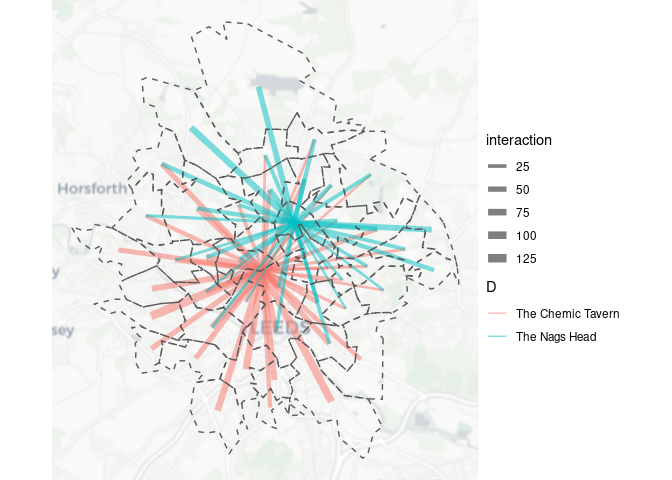
\includegraphics{main_files/figure-latex/pubresmap-1.pdf}
\caption{\label{fig:pubresmap}Results of a reproducible SIM undertaken on a minimal example based on synthetic data representing hypothetical trips to 2 pubs in Leeds, UK.}
\end{figure}

\hypertarget{calibration}{%
\section{Calibration}\label{calibration}}

As Openshaw (1975) succinctly puts it, ``calibration is the process of providing estimates of the unknown parameters we have identified as the independent variables of the model''.
In a basic gravity formulation of a spatial interaction model there will be three parameters to estimate relating to origin mass or emissivity, destination mass or attractiveness and a parameter determining the frictional effect of the cost of interactions occurring between the two.

The process of calibration allows the basic formulation of the model to be tweaked by adjusting the values of these parameters according to whatever context the model is being used in so that the estimates produced by the model correspond as closely as possible to any observations or data that a researcher might have.
In doing so, as well as producing better estimates from our model, we learn something about our system through the parameter values themselves.
For example, the one parameter that appears in all spatial interaction models relates to the cost exponent.
Almost universally described in the literature with the symbol \(\beta\) and almost always negative, the value of the beta parameter in a given system reveals the frictional effect that the cost of interaction has on the flows being observed, with higher negative values indicating a more severe deterrent.
Parameters associated with other variables, depending on the model, tell the story of the elements of the system and allow us to make judgements about what might be leading to the behaviours we observe -- why socio economic status may influence shopping expenditure, for example.

The big challenge is that calibration requires both data and -- particularly where there are multiple parameters to calibrate - software.
Forty or fifty years ago when many of the theoretical foundations of spatial interaction modelling were laid, the data landscape was somewhat different from today -- flow data were rarely available in volume and certainly not at the sort of temporal rhythm they are now where, for example, supermarket loyalty-card holders generate origin/destination revenue flow data from residential origins to store destinations at daily frequencies over time periods than can cover many years or even decades.
As such, we might be forgiven for expecting that even if the science and theory underpinning the models has not developed very much, the software and processes facilitating calibration -- relating empirical observations to the theoretical representations embodied in the models -- might have.
But in many ways, they have not.

Today it's not uncommon for flow data to be collected for various purposes.
As already mentioned it exists where any retailer has a loyalty card expenditure linked to a customer's home address and the store they shop in.
It exists in the public sector where, for example, school roll information is held with the home addresses of pupils.
It exists in the databases of companies like SafeGraph who derive trip data between homes and various point of interest destinations from mobile phone locational traces.
Accessing interaction data for a system of interest is not the barrier it once was, even if the proprietary nature of some of it can still present some access challenges.
However, for anyone who is in possession of these data, making sense of it -- understanding where commuting flows are unexpected, or why some retail stores of apparently similar composition have wildly different income profiles -- is more of a challenge.

Much of the challenge is because there is a dearth of knowledge through of a lack of exposure within geographical education.
Despite these models underpinning many of the processes that interest geographers, spatial interaction models are not taught to undergraduate geography students in the same way that, say, regression models are taught to economists or social psychologists.
As such, it is not immediately obvious, even for those coming out of geography degree programmes which might incorporate some level of `GIS' education, how anyone might go about fitting their spatial data to a theoretical model, calibrating the parameters and revealing properties of their system.

The question the follows, then, is why have cohorts of undergraduate geography students not been taught how to fit these models and explore systems of spatial interaction when it has been standard practice to show them how to produce choropleth maps on a computer or learn to apply a post-colonial lens to the interpretation of a text?
The answer has to come down to a problem of accessibility.
We discuss elsewhere in this chapter the fact that reproducibility has been an issue in the field, but that with packages like SPINT (*Oshan reference) and our own efforts with the simodels package in R, the tide is beginning to turn.
However, calibration remains a challenging sub-topic for reproducibility and the wider accessibility of these models, particularly where algorithms and routines which are able to calibrate parameters have remained locked away - either behind dense algebraic notation in dusty papers from the 1970s, or where they have found their way into software, behind paywalls as in the case of the Huff Model calibration routines found in ArcGIS but obscured to most behind the additional `Business Analyst' licence.

Ironically, perfectly effective calibration routines have been available for as long as students have been running regression models in their introductory statistics classes.
Occasional references can be found in the historic literature such as in papers by Fotheringham and Webber (1980) and Flowerdew and Aitken (1982) which lift the curtain and reveal that through reformulating the classic Wilsonian entropy maximising spatial interaction model as either a logged OLS regression model or a generalised linear model utilising a Poisson or negative binomial distributions, multiple parameters can be calibrated easily.
These models are all available in common statistical software packages and implement algorithms such as iteratively reweighted least squares to find the maximum likelihood parameter values, but for most trying to make sense of the field coming across papers by some of the doyens (for it was and still is a male-dominated field) of the scene such as Wilson, Fotheringham, Pooler, Openshaw and Roy, while undoubtedly mathematically and theoretically rigorous, notes on calibration were at best reduced to a passing reference to `least squares' or at worst a lengthy derivation of maximum likelihood of Newton Raphson methods.

Compounding the calibration challenge further, myriad proprietary data formats emerged during the 1980s and 90s with rarely the same file-type used for `GIS' analysis as statistical modelling.
~A melange that has meant that for many the overheads involved just in converting data between SPSS, Minitab, Stata, ArcGIS, MapInfo will have been too severe to contemplate.
Even for those fortunate enough to have received a grounding in both spatial analysis methods and more general statistical techniques this will have not helped any mental balkanisation perhaps already occurring through a lack of practical education where regression may have been taught entirely separately from spatial modelling.

Calibration is at the centre of what makes spatial interaction models useful to researchers and we have outlined why challenges emerged and persisted in the field.
But we are confident that with software such as R and Python meaning that statistical and geographic analyses are no longer separated in the workflow and packages emerging, contributed to by researchers active in the field enabling others to run reproducible analyses, these challenges need not persist.
With increasing volumes of data coming online to allow multiple different sorts of models to be tested and calibrated against empirical observations in a variety of different contexts, we will be able to find solutions to problems that inevitably emerge when calibrating general models to messy reality: issues of sparse or huge interaction matrices.
Issues of multiple scales, dimensions and aggregations.
Issues of spatial non-stationarity.
Issues of incomplete, poor or otherwise imperfect calibration data.
These are all problems that persist but that due to new researchers in the field invariably starting from scratch rather than usefully building on existing knowledge through accessible methods, have not yet been successfully solved.

\hypertarget{expanding-spatial-interaction-modelling}{%
\section{Expanding spatial interaction modelling}\label{expanding-spatial-interaction-modelling}}

Objective of the section: To discuss ways in which spatial interaction modelling can be expanded.
I am particularly interested in advocating for (1) seeing spatial interaction models in a context of uncertainty, rather than as mathematical models; and, (2) discussing how hierarchical / generalised linear mixed modelling can offer ways to capture variability across places and populations.

\hypertarget{spatial-interaction-modelling-using-machine-learning}{%
\section{Spatial interaction modelling using machine learning}\label{spatial-interaction-modelling-using-machine-learning}}

Objective of the section: To discuss how machine learning can enhance flow count inference and prediction

\hypertarget{facilitating-future-progress-of-spatial-interaction-modelling}{%
\section{Facilitating future progress of spatial interaction modelling}\label{facilitating-future-progress-of-spatial-interaction-modelling}}

Objective of the section: To identify and discuss the key pillars that will enable progress on all the proposed fronts - open science, important and new questions and digital infrastructure.
I see this as our conclusion - probably one or two short paragraph summarising what has been discussed with a forward looking approach.

These are the challenges.
We therefore need software to enhance reproducibility, calibration, - deal with issues of scalability, multiples scales, spatial non-stationarity,

\hypertarget{references}{%
\section*{References}\label{references}}
\addcontentsline{toc}{section}{References}

\hypertarget{refs}{}
\begin{CSLReferences}{1}{0}
\leavevmode\vadjust pre{\hypertarget{ref-dennett_modelling_2018}{}}%
Dennett, Adam. 2018. {``Modelling Population Flows Using Spatial Interaction Models.''} \emph{Australian Population Studies} 2 (2): 33--58. \url{https://doi.org/10.37970/aps.v2i2.38}.

\leavevmode\vadjust pre{\hypertarget{ref-niedomysl2017}{}}%
Niedomysl, Thomas, Ola Hall, Maria Francisca Archila Bustos, and Ulf Ernstson. 2017. {``Using Satellite Data on Nighttime Lights Intensity to Estimate Contemporary Human Migration Distances.''} \emph{Annals of the American Association of Geographers} 107 (3): 591--605. \url{https://doi.org/10.1080/24694452.2016.1270191}.

\leavevmode\vadjust pre{\hypertarget{ref-nust_practical_2021}{}}%
Nüst, Daniel, and Edzer Pebesma. 2021. {``Practical Reproducibility in Geography and Geosciences.''} \emph{Annals of the American Association of Geographers} 111 (5): 1300--1310. \url{https://doi.org/10.1080/24694452.2020.1806028}.

\leavevmode\vadjust pre{\hypertarget{ref-ogcopengeospatialconsortiuminc_opengis_2011}{}}%
(OGC) Open Geospatial Consortium Inc. 2011. {``OpenGIS Implementation Specification for Geographic Information - Simple Feature Access - Part 1: Common Architecture.''} \url{https://www.ogc.org/standards/sfa}.

\leavevmode\vadjust pre{\hypertarget{ref-oshan2021spatial}{}}%
Oshan, Taylor M. 2021. {``The Spatial Structure Debate in Spatial Interaction Modeling: 50 Years On.''} \emph{Progress in Human Geography} 45 (5): 925--50.

\leavevmode\vadjust pre{\hypertarget{ref-popper_logic_1934}{}}%
Popper, Karl. 1934. \emph{The Logic of Scientific Discovery}. Hutchinson. \url{http://books.google.com/books?id=MdvaSAAACAAJ\&pgis=1}.

\leavevmode\vadjust pre{\hypertarget{ref-rodrigue_geography_2013}{}}%
Rodrigue, Jean-Paul, Claude Comtois, and Brian Slack. 2013. \emph{The Geography of Transport Systems}. 3 edition. London ; New York: Routledge.

\leavevmode\vadjust pre{\hypertarget{ref-schwartz1973interpreting}{}}%
Schwartz, Aba. 1973. {``Interpreting the Effect of Distance on Migration.''} \emph{Journal of Political Economy} 81 (5): 1153--69.

\leavevmode\vadjust pre{\hypertarget{ref-simini_universal_2012}{}}%
Simini, Filippo, Marta C González, Amos Maritan, and Albert-László Barabási. 2012. {``A Universal Model for Mobility and Migration Patterns.''} \emph{Nature}, February, 812. \url{https://doi.org/10.1038/nature10856}.

\leavevmode\vadjust pre{\hypertarget{ref-wilson_family_1971}{}}%
Wilson, AG. 1971. {``A Family of Spatial Interaction Models, and Associated Developments.''} \emph{Environment and Planning} 3 (January): 132. https://doi.org/\url{https://doi.org/10.1068/a030001}.

\end{CSLReferences}




% print the bibliography
\setlength{\bibsep}{0.00cm plus 0.05cm} % no space between items
\bibliographystyle{apalike}
\bibliography{sim_refs}



\end{document}
